\section{Timetable}
\label{section:timetable}
In figure \ref{fig:timetable}, the preliminary time frame of this project is displayed. The project is mainly scheduled on a weekly basis, with week 1 starting February 3rd. As described in section \ref{section:methodology}, the project is also partitioned into sprints according to the scrum methodology, with the first sprint starting on project week 3. As each sprint is planned on the basis of the current state of the project, the user stories and tasks of the sprints are not marked in the timetable.

Scheduled deadlines are for each row marked with their specified due date within the week of the deadline. Non-dated milestones are implicitly due at the end of their respective week or sprint, and marked as the far right of the boxes of each row. The progress of the thesis is partitioned into three iterations, a first and second draft, as well as the final edit. Likewise, the progress of the developed platform is also partitioned into three iterations, resulting a first and second prototype before the final product. 

\begin{figure}[H]
    \centering
    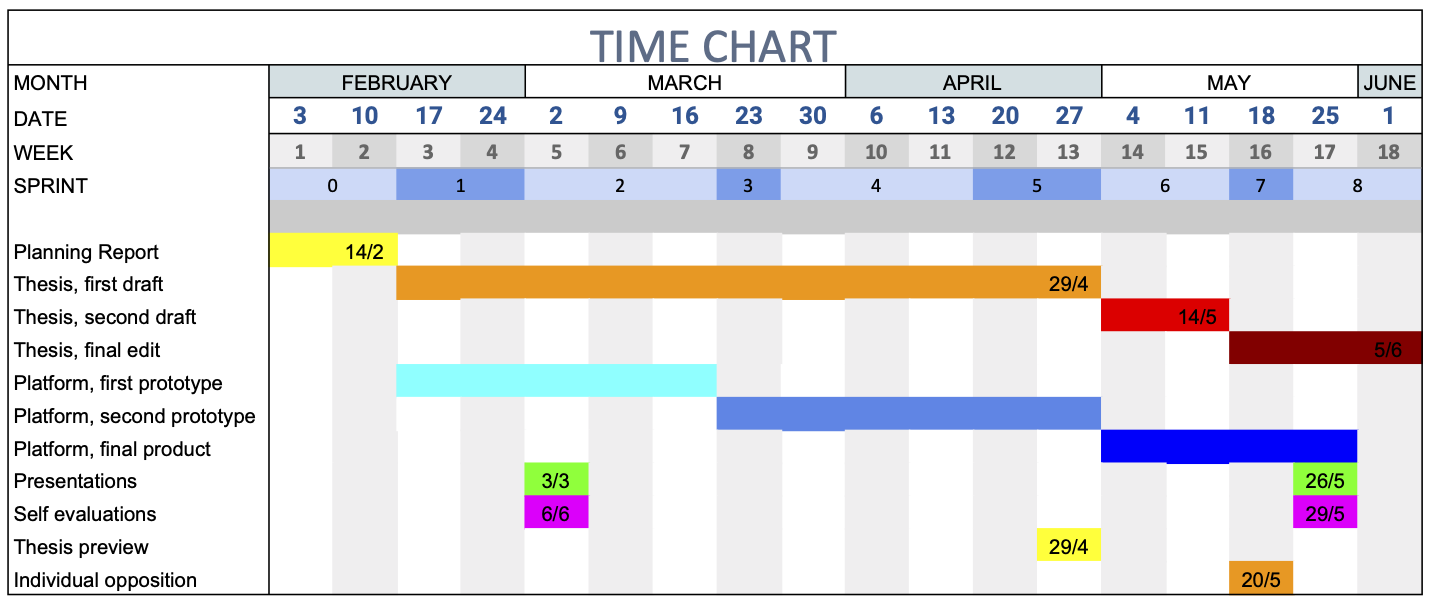
\includegraphics[width = \textwidth]{Planning report/images/timetable.png}
    \caption{The preliminary timetable of the thesis project.}
    \label{fig:timetable}
\end{figure}